
%(BEGIN_QUESTION)
% Copyright 2013, Tony R. Kuphaldt, released under the Creative Commons Attribution License (v 1.0)
% This means you may do almost anything with this work of mine, so long as you give me proper credit

This Ethernet network has a problem in it somewhere:

$$\includegraphics[width=15.5cm]{i03547x01.eps}$$

\begin{itemize}
\item{} 1 can ``ping'' 5
\item{} 3 can ``ping'' {\tt www.google.com}
\item{} 2 can ``ping'' 5 
\item{} 4 cannot ``ping'' {\tt www.bing.com}
\end{itemize}

Identify the likelihood of each specified fault for this network.  Consider each fault one at a time (i.e. no coincidental faults), determining whether or not each fault could independently account for {\it all} measurements and symptoms in this network.

% No blank lines allowed between lines of an \halign structure!
% I use comments (%) instead, so that TeX doesn't choke.

$$\vbox{\offinterlineskip
\halign{\strut
\vrule \quad\hfil # \ \hfil & 
\vrule \quad\hfil # \ \hfil & 
\vrule \quad\hfil # \ \hfil \vrule \cr
\noalign{\hrule}
%
% First row
{\bf Fault} & {\bf Possible} & {\bf Impossible} \cr
%
\noalign{\hrule}
%
% Another row
Router failed &  &  \cr
%
\noalign{\hrule}
%
% Another row
Internet service provider failed &  &  \cr
%
\noalign{\hrule}
%
% Another row
Cable failed between computer \#1 and Hub A &  &  \cr
%
\noalign{\hrule}
%
% Another row
Cable failed between computer \#2 and Hub A &  &  \cr
%
\noalign{\hrule}
%
% Another row
Cable failed between computer \#4 and Hub B &  &  \cr
%
\noalign{\hrule}
%
% Another row
Cable failed between computer \#5 and Hub B &  &  \cr
%
\noalign{\hrule}
%
% Another row
Cable failed between Hub A and Router &  &  \cr
%
\noalign{\hrule}
%
% Another row
Cable failed between Hub B and Router &  &  \cr
%
\noalign{\hrule}
%
% Another row
Server failed at {\tt www.google.com} &  &  \cr
%
\noalign{\hrule}
%
% Another row
Server failed at {\tt www.bing.com} &  &  \cr
%
\noalign{\hrule}
} % End of \halign 
}$$ % End of \vbox

\underbar{file i03547}
%(END_QUESTION)





%(BEGIN_ANSWER)

% No blank lines allowed between lines of an \halign structure!
% I use comments (%) instead, so that TeX doesn't choke.

$$\vbox{\offinterlineskip
\halign{\strut
\vrule \quad\hfil # \ \hfil & 
\vrule \quad\hfil # \ \hfil & 
\vrule \quad\hfil # \ \hfil \vrule \cr
\noalign{\hrule}
%
% First row
{\bf Fault} & {\bf Possible} & {\bf Impossible} \cr
%
\noalign{\hrule}
%
% Another row
Router failed &  & $\surd$ \cr
%
\noalign{\hrule}
%
% Another row
Internet service provider failed &  & $\surd$ \cr
%
\noalign{\hrule}
%
% Another row
Cable failed between computer \#1 and Hub A &  & $\surd$ \cr
%
\noalign{\hrule}
%
% Another row
Cable failed between computer \#2 and Hub A &  & $\surd$ \cr
%
\noalign{\hrule}
%
% Another row
Cable failed between computer \#4 and Hub B & $\surd$ &  \cr
%
\noalign{\hrule}
%
% Another row
Cable failed between computer \#5 and Hub B &  & $\surd$ \cr
%
\noalign{\hrule}
%
% Another row
Cable failed between Hub A and Router &  & $\surd$ \cr
%
\noalign{\hrule}
%
% Another row
Cable failed between Hub B and Router &  & $\surd$ \cr
%
\noalign{\hrule}
%
% Another row
Server failed at {\tt www.google.com} &  & $\surd$ \cr
%
\noalign{\hrule}
%
% Another row
Server failed at {\tt www.bing.com} & $\surd$ &  \cr
%
\noalign{\hrule}
} % End of \halign 
}$$ % End of \vbox

%(END_ANSWER)





%(BEGIN_NOTES)

{\bf This question is intended for exams only and not worksheets!}.

%(END_NOTES)


